\documentclass[italian]{beamer}
\usecolortheme{beaver}
\useoutertheme{infolines}
\usetheme{CambridgeUS}
\setbeamertemplate{navigation symbols}{\insertframenumber} 
\usepackage{pstricks}
\usepackage[tight,nice]{units}
\usepackage[]{url}
\usepackage{babel}
\usepackage[]{graphicx}
\usepackage[utf8x]{inputenc}
\usepackage[T1]{fontenc}
\usepackage{ae,aecompl}
\usepackage{nicefrac}
\include{pst-plot}
\include{pst-3d}
\newtheorem{definizione}{Definizione}
\frenchspacing
\pagestyle{empty}
\title{Discriminazione dei muoni da decadimenti di B e D}
\author{Matteo Abis \\
\url{matteo@latinblog.org}}
\institute{Università degli Studi di Padova\\
Scuola Galileiana di Studi Superiori}
\date{\today}
\begin{document}
\begin{frame}
    \titlepage
\end{frame}

\begin{frame}{Dati Monte Carlo}{un milione di eventi $pp \to \mu X$}
Tagli sulle tracce ricostruite:
\begin{itemize}
    \item identificazione dei muoni \emph{TMLastStationOptimizedLowPtTight}:
        \begin{itemize}
            \item hit nell'ultima camera a $\mu$
            \item almeno due segmenti compatibili nelle camere a $\mu$
            \item segmenti nel \emph{tracker} ben accoppiati con i segmenti
                nelle camere a $\mu$
        \end{itemize}
    \item $p_t > \unit[3]{GeV/c}$
    \item $|\eta| < 2.5$
\end{itemize}
\end{frame}

\begin{frame}{Associazione tracce ricostruite $\to$ particelle generate}
\begin{itemize}
    \item minima distanza nello spazio $(\eta, \phi)$. $\Delta R =
        \sqrt{\Delta \eta^{2} + \Delta \phi^{2}}$
    \item ulteriore taglio delle coppie con $\Delta R < 0.1$ o $\Delta p_t /
        p_t < 0.1$
\end{itemize}
\begin{figure}[h]
    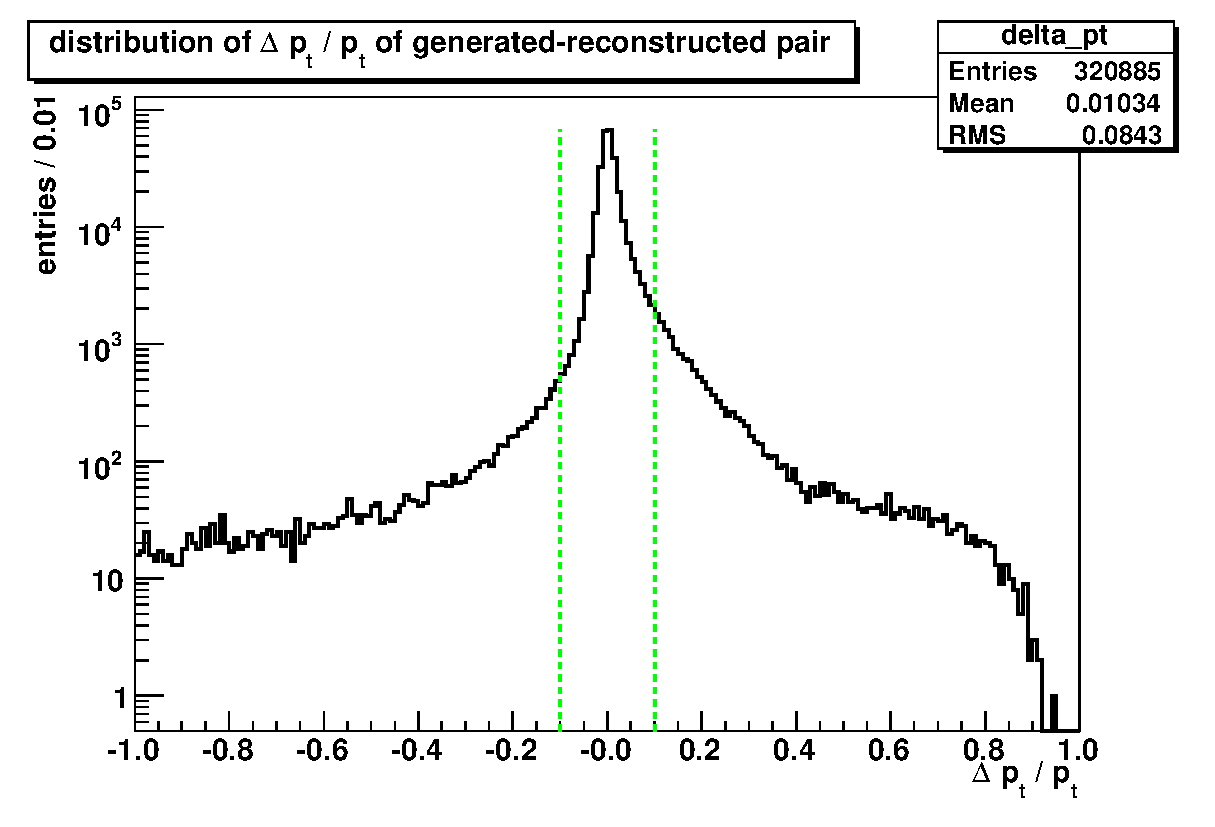
\includegraphics[width=0.5\textwidth]{crea_istogrammi/delta_pt.eps}
    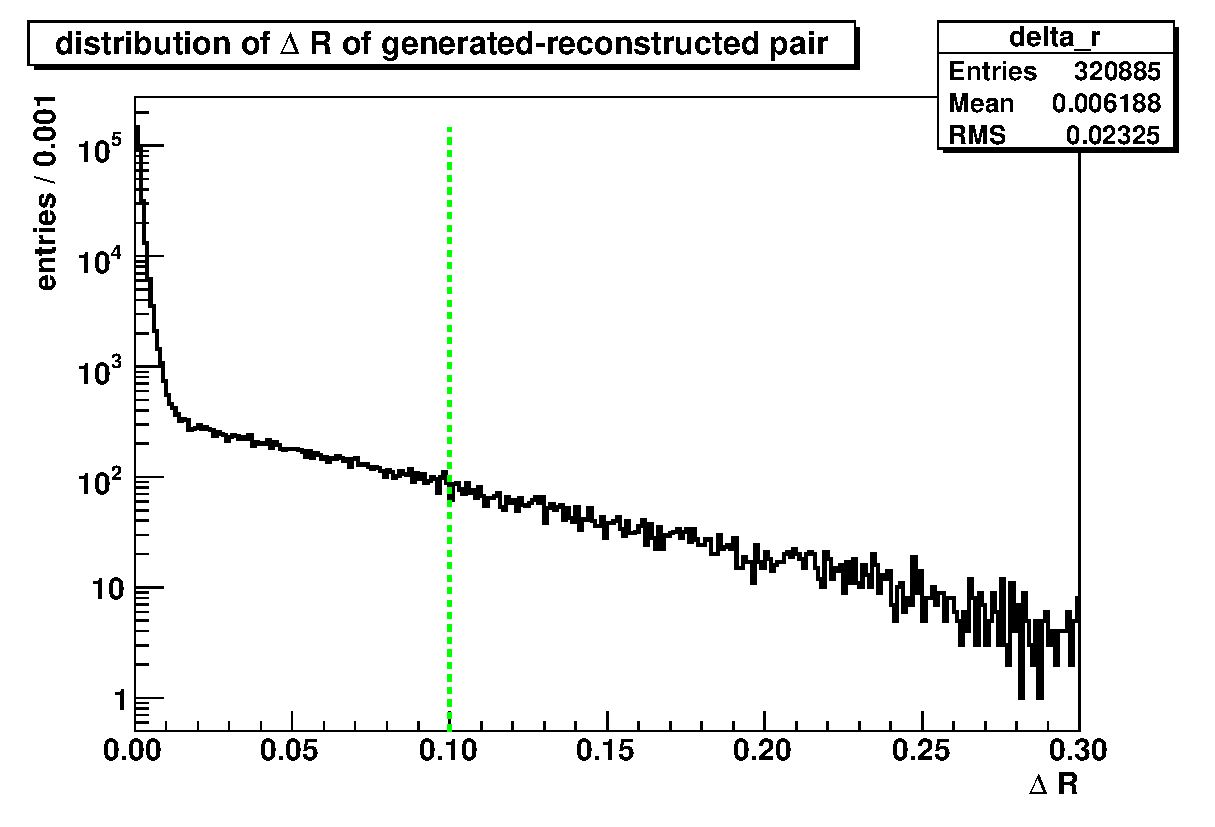
\includegraphics[width=0.5\textwidth]{crea_istogrammi/delta_r.eps}
\end{figure}
\end{frame}

\begin{frame}{\emph{circolare} o \emph{lineare}}{prima ipotesi di studio sul
    parametro d'impatto $d$}
    \begin{block}{algoritmo CMSSW 2.2.9}
        \begin{itemize}
            \item traccia circolare $\to$ $RP$
            \item dxy(PV) $\to$ lineare da $RP$
        \end{itemize}
    \end{block}
\begin{figure}[h]
    \psset{unit=0.8}
    \begin{pspicture*}(-1,-1)(4,4)
        \psaxes*[labels=none,ticks=none,linewidth=.6pt]{->}(0,0)(-1,-1)(4,4)      
        \psellipticarc[]{<-}(5,2)(3.5,3.5){150}{180}
        \psellipticarc[linestyle=dashed,dash=0.2 0.15]{}(5,2)(3.5,3.5){180}{240}
        \psline[linewidth=0.8pt,linestyle=dashed,dash=0.1 0.1]{}(0,0)(1.75, 0.7)
        \uput*[30](0.28, 0.25){\tiny{dxy()}}
        \psdot*(0, 0)
        \uput[225](0, 0){\small O}
        \psplot[plotstyle=curve]{-1}{6.3}{x -2.5 mul 5.075 add}
        \psdot*(-0.5,2)
        \psdot*(1.75,0.7)
        \uput[45](1.75, 0.7){\small{RP}}
        \uput[225](-0.48, 2){\small{PV}}
        \psline[linewidth=0.8pt,linestyle=dashed,dash=0.1 0.1]{}(-.5,2)(1, 2.6)
        \uput*[30](-0.58, 2.55){\tiny{dxy(PV)}}
        \rput[r]{*0}(-0.2, 3.8){$y$}
        \rput[l]{*0}(2.1, 3){\small{traccia}}
        \rput[t]{*0}(3.8, -0.2){$x$}
    \end{pspicture*}
\end{figure}
\end{frame}
    \begin{frame}
        {studio della risoluzione su $d$, gen--reco}
        GenParticle non ha un metodo per $d$
        \begin{itemize}
            \item C. Favaro $\to$ estrapolazione lineare
            \item P. Bortignon $\to$ estrapolazione circolare
        \end{itemize}
    \end{frame}

\begin{frame}
    {circolare anche su reco::Particle?}
    $d$ fino a $\unit[4]{m}$
\begin{figure}[h]
    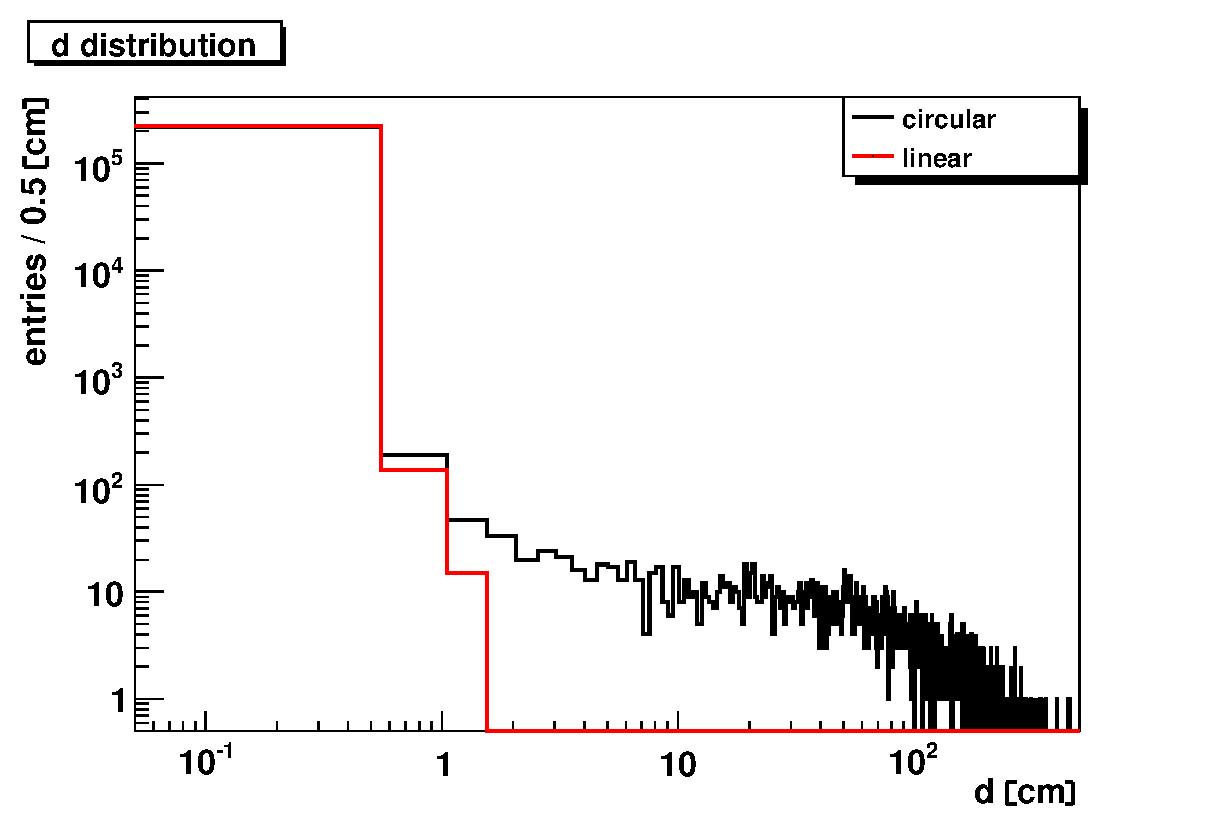
\includegraphics[width=0.7\textwidth]{crea_istogrammi/glob_inn.eps}
\end{figure}
\end{frame}

\begin{frame}
    {Muon::vertex() e Muon::track()}
    {che cosa restituiscono?}
    Muon.h $\to$ tre tipi di traccia:
    \begin{description}
        \item[Muon::innerTrack()] solo \emph{hit} nel \emph{tracker}
        \item[Muon::outerTrack()] solo \emph{hit} nelle camere a $\mu$
        \item[Muon::globalTrack()] \emph{tracker} + $\mu$
    \end{description}

    \begin{block}
        {Attenzione!}
        \begin{itemize}
            \item muon->track() $=$ muon->innerTrack()
            \item muon->vertex() $=$ muon->globalTrack()->vertex()
        \end{itemize}
    \end{block}
\end{frame}

\begin{frame}
    {pat::Muon sfugge alla gerarchia di CMSSW}
    \begin{itemize}
        \item reco::Particle e reco::TrackBase non sono imparentate
        \item reco::Particle è costruita da variabili cinematiche di
            \emph{track}
        \item pat::Muon eredita da reco::Particle, ma ha tre tracce.
        \item accedere alle variabili dei $\mu$ senza passare da una delle
            \emph{track} genera ambiguità.
    \end{itemize}
\end{frame}
    
\begin{frame}
    {lineare $=$ circolare}
    La coda con $d$ fino a \unit[4]{m} era dovuta non all'approssimazione
    circolare, ma all'uso di parametri cinematici da \emph{globalTrack}.
\begin{figure}[h]
    \includegraphics[width=0.7\textwidth]{crea_istogrammi/glob_inn2.eps}
\end{figure}
\end{frame}

\begin{frame}
    {lineare $=$ circolare}
    \begin{table}[h]
        \centering
        \begin{tabular}{rcc}
            traccia & \unit[media]{(pm)}& \unit[RMS]{(pm)}\\
            global & -0.136 & 5.189\\
            inner & -0.094 & 4.418\\
        \end{tabular}
    \end{table}
\begin{figure}[h]
    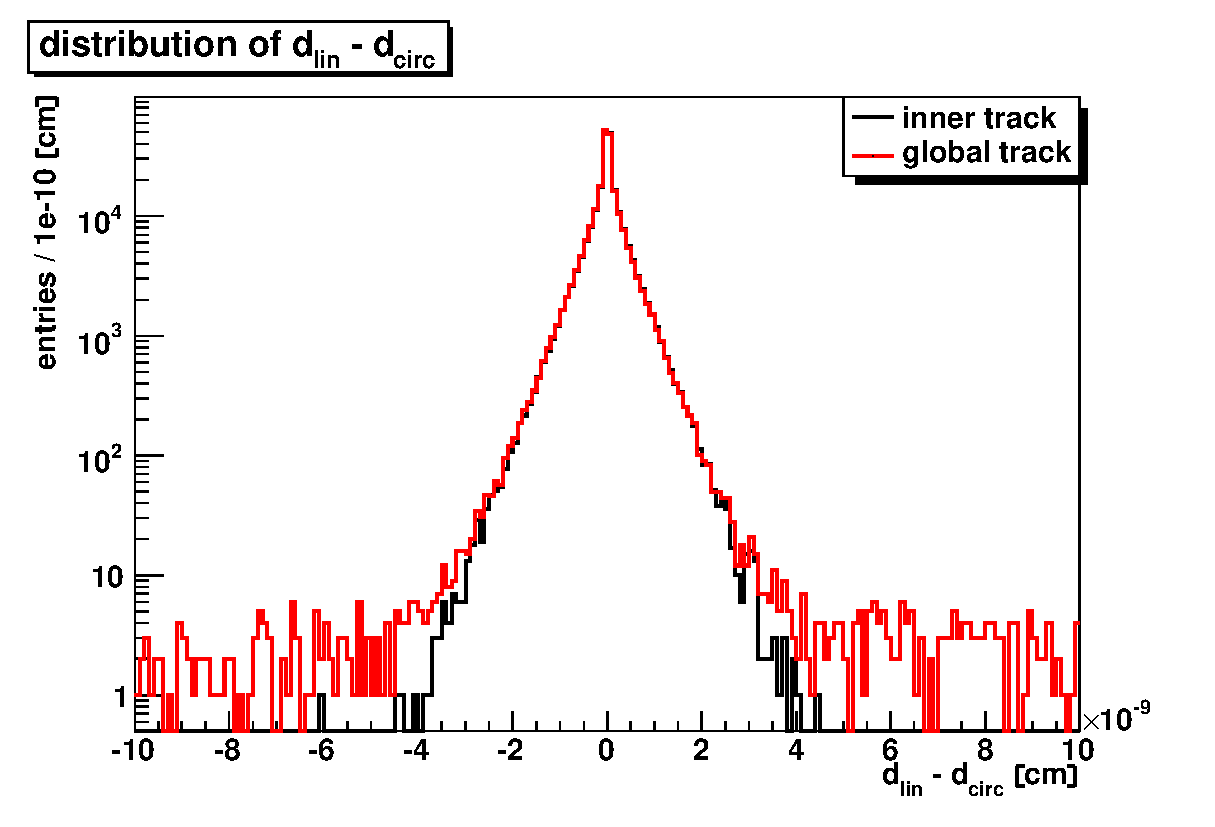
\includegraphics[width=0.6\textwidth]{crea_istogrammi/lin_circ.eps}
\end{figure}
976 \emph{under/overflow} per le \emph{global}, 938 entro
$\unit[10^{-5}]{cm}$
\end{frame}

\begin{frame}{Distribuzioni in $d$}
Parametri analizzati:
\begin{itemize}
    \item \emph{global track} e \emph{inner track}
    \item $p_t$ minimo
    \item luminosità integrata (numero di eventi)
\end{itemize}
\begin{figure}[h]
    \includegraphics[width=0.5\textwidth]{crea_istogrammi/d_lin_inner.eps}
    \includegraphics[width=0.5\textwidth]{crea_istogrammi/d_lin_global.eps}
\end{figure}
\end{frame}
\begin{frame}{Test di Kolmogorov-Smirnov}
    \begin{block}{}
        probabilità che due campioni provengano dalla stessa popolazione
    \end{block}

    \begin{block}{in funzione del numero di eventi (taglio 
        $p_t > \unit[3]{GeV/c}$)}
    $5\sigma \to \unit[7\cdot 10^{-3}]{pb^{-1}}$ ($\approx$
    \unit[250 000]{$\mu$}) 
    \end{block}
    
\begin{figure}[h]
    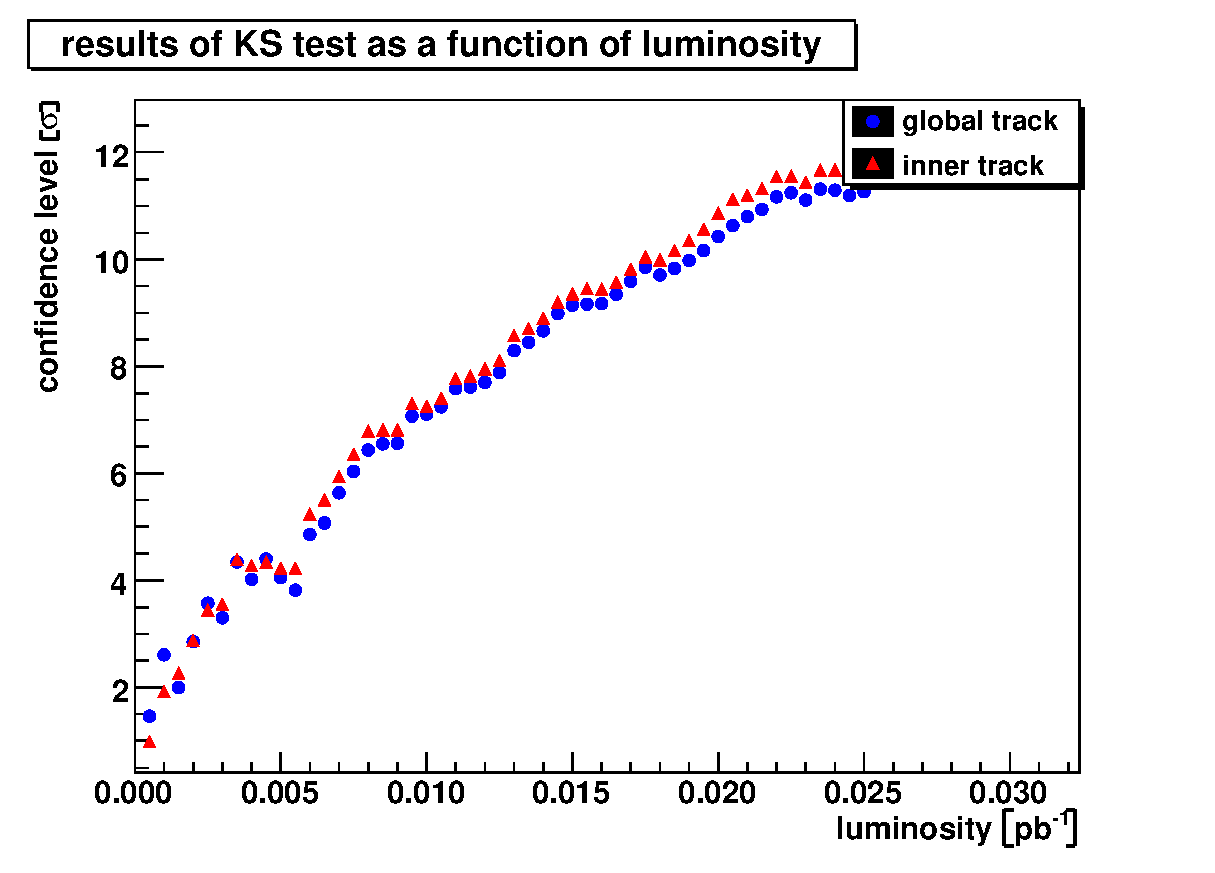
\includegraphics[width=0.6\textwidth]{crea_istogrammi/lum_1.eps}
\end{figure}
\end{frame}

\begin{frame}{Taglio in $p_t$}
    il livello di confidenza scende perch\'e diminuisce la significanza
    statistica del campione.
\begin{figure}[h]
    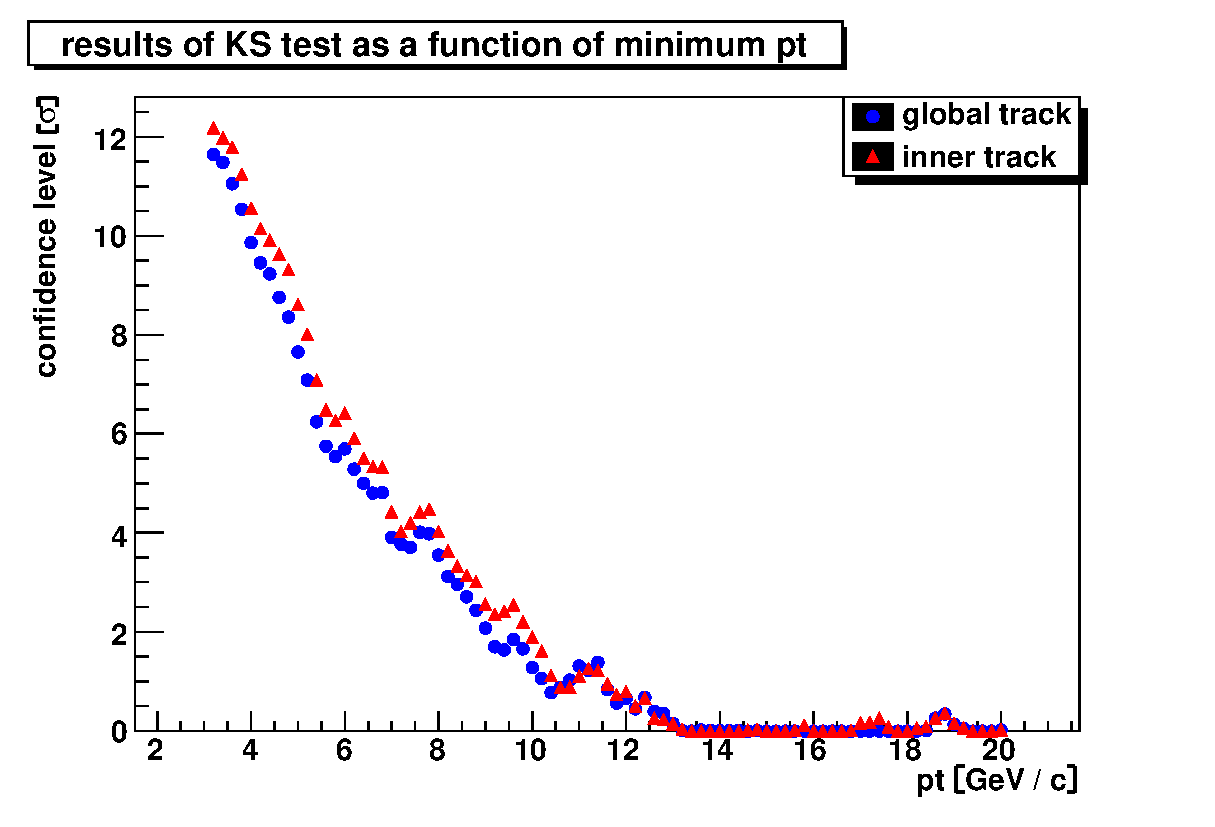
\includegraphics[width=0.7\textwidth]{crea_istogrammi/pt_1.eps}
\end{figure}
\end{frame}
\begin{frame}{Pseudo-esperimenti}{eliminare la dipendenza dal numero di
    eventi}
    \begin{itemize}
        \item<+-> distribuzione $d$ dei $\mu$ che superano il taglio richiesto
        \item<+-> due istogrammi da 10000 GetRandom dalle distribuzioni
        \item<+-> test di Kolmogorov
        \item<+-> si ripete 100 volte, media e RMS sul grafico 
    \end{itemize}
\begin{figure}[h]
    \includegraphics<+->[height=0.6\textheight]{crea_istogrammi/pseudo_pt_1.eps}
\end{figure}
\end{frame}

\begin{frame}{Conclusioni} 
    \begin{itemize}
        \item l'approssimazione lineare è ottima ($PV \approx O$)
        \item \emph{inner track} discrimina meglio di \emph{global track}
        \item luminosità integrata $\to 5\sigma$: $\unit[7\cdot
            10^{-3}]{pb^{-1}} \approx$ 1--12 giorni di
            LHC\footnote{Stima della luminosità istantanea tra
            $\unit[10^{30}]{cm^{-2}s^{-1}}$ e $\unit[10^{31}]{cm^{-2}s^{-1}}$}. 
        \item taglio più alto in $p_t$ non sembra migliorare la discriminazione
    \end{itemize}
\end{frame}

\end{document}
